\scanpage{21}
On a de plus un foncteur \uline{pleinement fidèle}
\diagram{\begin{tikzcd} C \arrow[r] & \uline{\operatorname{Rep}}(\mathcal G) \end{tikzcd}}
\margin{NB. on a\par
\diagram{\begin{tikzcd}
C\times\mathcal G \arrow[r] \arrow[d,no head] & \uuline{\operatorname{Mod}} \\
\begin{array}{c}\text{\unsure{catég.} fibrée \unsure{constante}}\\\text{de val. }C\end{array} &
\end{tikzcd}}}
dont l'image est formée des représentations de $\mathcal G$ qui \inserted{sont ``de degré $1$'' et sont} \uline{localement} \deleted{sont} de degré donné $n(x)$ (où $n(x)$ est la fonction \unsure{rg} de ${}_A O$ sur $\operatorname{Spec}A$ \ldots).

Donc on trouve

Une catégorie de Deuring-Azumaya sur $A$ est ess\textsuperscript{t} la même chose qu'une gerbe sur $S=\operatorname{Spec}A$, de lien $G_m$, \uline{munie} d'une fonction $x\longmapsto n(x)$ loc. constante sur $\operatorname{Spec}A$, avec \unsure{$k$} $n(x)$ tel que

a) la gerbe soit \deleted{\unsure{d'un rang}\ \unsure{alors}} réalisable globalement par une algèbre d'Azumaya de rang $n(x)$ \deleted{partout} en chaque pt \deleted{(ce qui est}\inserted{(mais cette algèbre n'est pas} déterminée)

\margin{On peut donc définir $\det X$ pour $X\in\operatorname{Ob}C$, comme un objet de $\operatorname{Rep}(\mathcal G)$. Si $X'=P\unsure{\otimes_O|\otimes_O^a}X$, on aura alors un isom $\det X'\simeq\det(X)\operatorname{Nrd}(P)$ où $\operatorname{Nrd}$ est la norme réduite, qu'on peut considérer comme foncteur\par
\diagram{\begin{tikzcd}
\operatorname{Mod.inv.}(O)\ \unsure{\text{drt.}} \arrow[r] & \operatorname{Mod.inv.}(A)
\end{tikzcd}}}

\figure{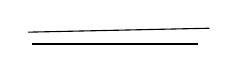
\begin{tikzpicture}\draw (0,0.05)--(2.3,0.10);\draw (0.05,-0.10)--(2.15,-0.10);\end{tikzpicture}}

Supposons qu'on ait une catégorie de Deuring \deleted{\unsure{stricte}} sur $A$ \deleted{anneau, tel que de Dedekind,} \inserted{normal, avec $O$ \deleted{\unsure{de rang}} \unsure{fin.} sur $A$ sans torsion et $O_K$ azumaya sur $K$.}
$U\subset S$ le plus grand ouvert sur lequel les $O=\uline{\operatorname{End}}(X)$ (un, tous, c'est kif-kif) soient d'Azumaya. Donc $C$ définit une gerbe \inserted{$\mathcal G_U$} de lien $G_m$ sur $U$, dont la classe dans $\operatorname{Br}(U)$ est tuée par $n$, \inserted{par le ``rang'' de $C$.} et $C\otimes_A\underset{A'}{\uline{\Gamma(U)}}$ se récupère par cette gerbe $\mathcal G_U$, à équivalence canonique (définie à isom uniques) près, \deleted{comme} la catégorie des repr. de cette
\mspage{20}
